\frame{
\begin{tikzpicture}[remember picture,overlay]
\fill[blue1]
(current page.north west) rectangle ([xshift=0.24\paperwidth,yshift=0.33\paperheight]current page.west|-{pic cs:end});
\end{tikzpicture}

\begin{textblock}{0.5}(0.02,0.03)
	\textcolor{white}{
		\Large Granular flows}
\end{textblock}


%% GRANUALR FLOWS
\begin{textblock}{0.95}(0.03,0.12)
	\textcolor{red}{rough structure - replace text by images:}
	
	1. Motivate physical system of granular flow
	(nice challenge to study)\\
	2. Motivate technique of radiography
	
	\begin{itemize}
		\item Granular flows - fluidized bed reactors
		\item optically opaque
		\item X-ray reveal the inside
		\item Tomography: full 3D information - but slow (no dynamics)
		\item Radiography: single projections - knowledge on imaging physics
		\item Here two techniques to quantify: densities \& dynamics
	\end{itemize}
\end{textblock}	


}
\note{hallo is this a note?}

%% OPAQUE
\frame{
	\begin{tikzpicture}[remember picture,overlay]
	\fill[blue1]
	(current page.north west) rectangle ([xshift=12.cm,yshift=-10.cm]current page.east|-{pic cs:end});
	\end{tikzpicture}
	\frametitle{\textcolor{white}{Particulate flows are \textbf{opaque}}}
	\begin{textblock}{0.9}(0.05,0.05)
		\centering
		\Large{
			\textcolor{white}{Particulate flows are \textbf{opaque}}}
	\end{textblock}

	\begin{textblock}{0.9}(0.05,0.15)
		\centering
		\movie[width =0.3\textwidth,loop]
		{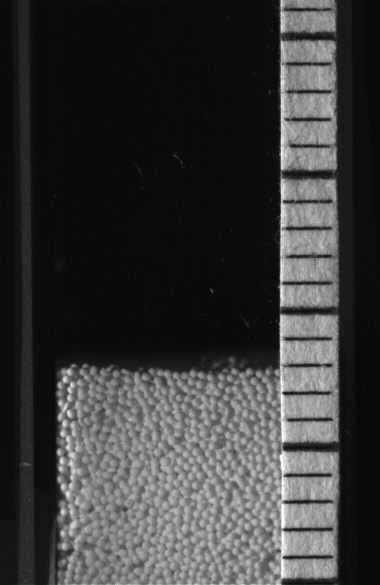
\includegraphics[width=0.3\textwidth]{Sources/motivation/video_welm_paetzold.png}}	
		{Sources/motivation/video_welm_paetzold.avi}
		
		\textcolor{white}{\footnotesize Master thesis Welm Pätzold}
	\end{textblock}
}


%% X-RAY RADIOGRAPHY
\frame{
\begin{tikzpicture}[remember picture,overlay]
\fill[blue1]
(current page.north west) rectangle ([xshift=0.28\paperwidth,yshift=0.33\paperheight]current page.west|-{pic cs:end});
\end{tikzpicture}

\begin{textblock}{0.5}(0.02,0.03)
	\textcolor{white}{
		\Large X-ray radiography}
\end{textblock}

\begin{textblock}{0.7}(0.02,0.05)
	\centering
	\only<1>{
	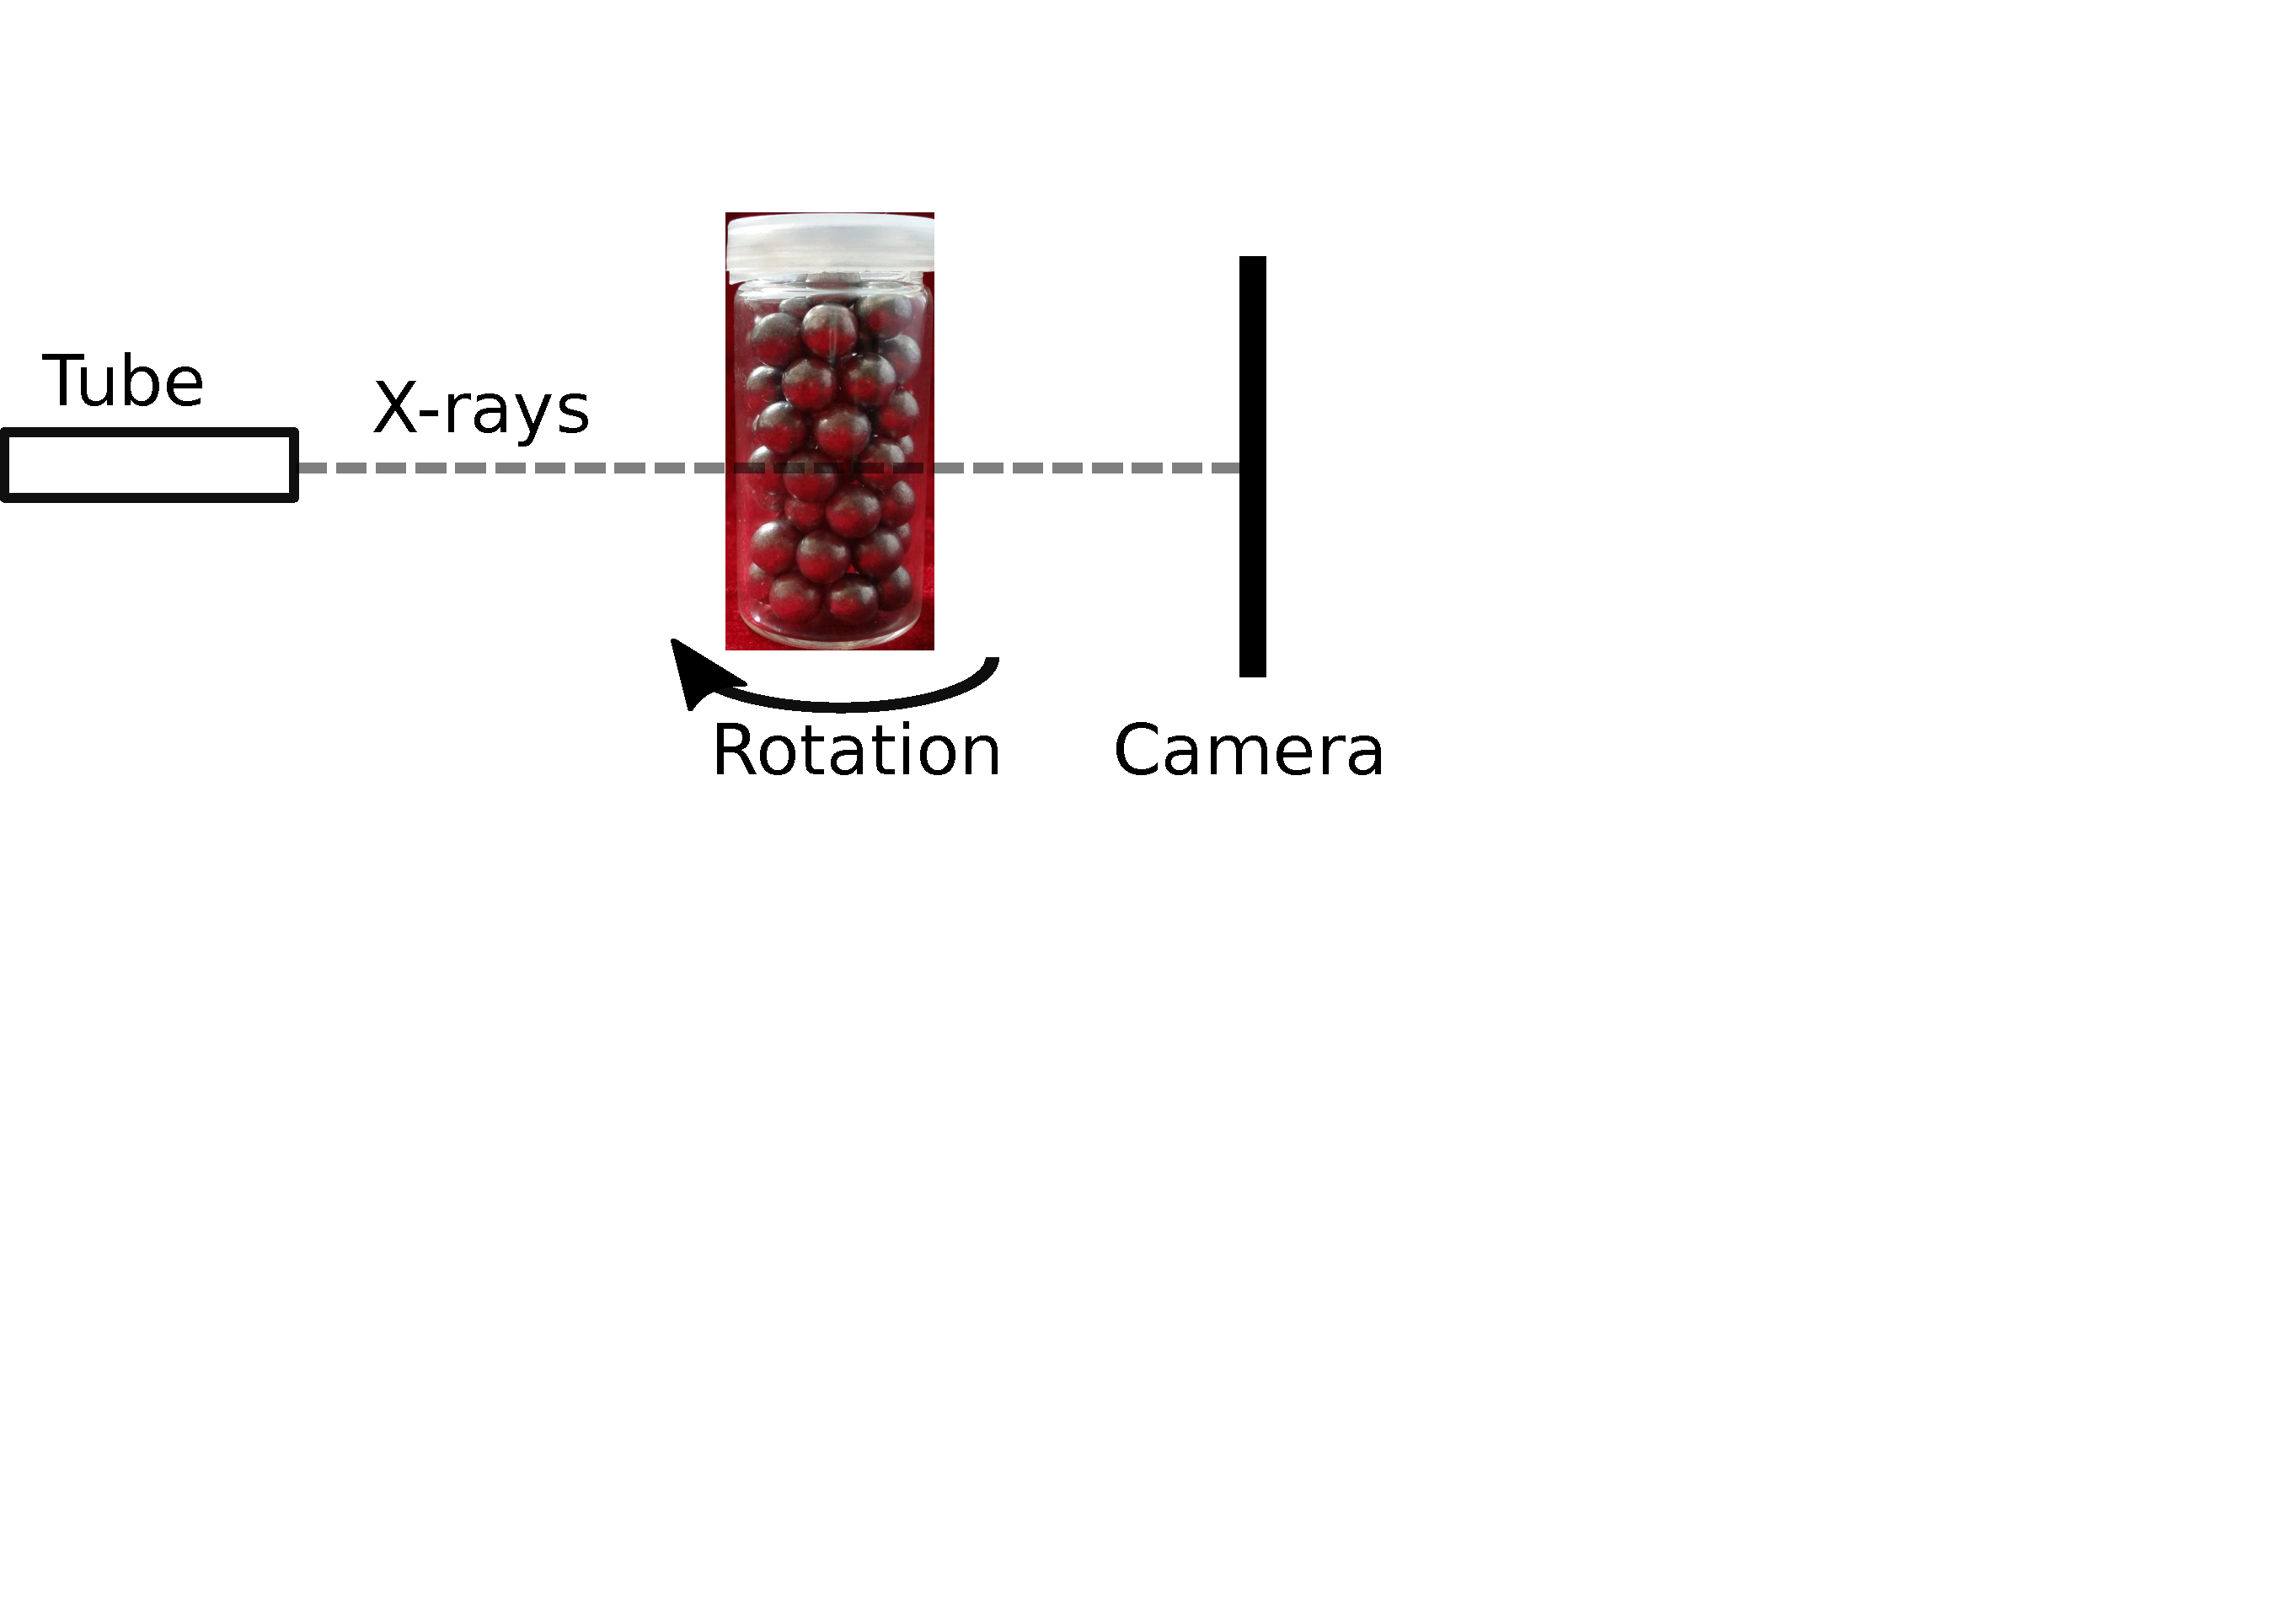
\includegraphics[width=\textwidth]{Sources/motivation/x-ray_setup_use0.pdf}}
	\visible<2->{
	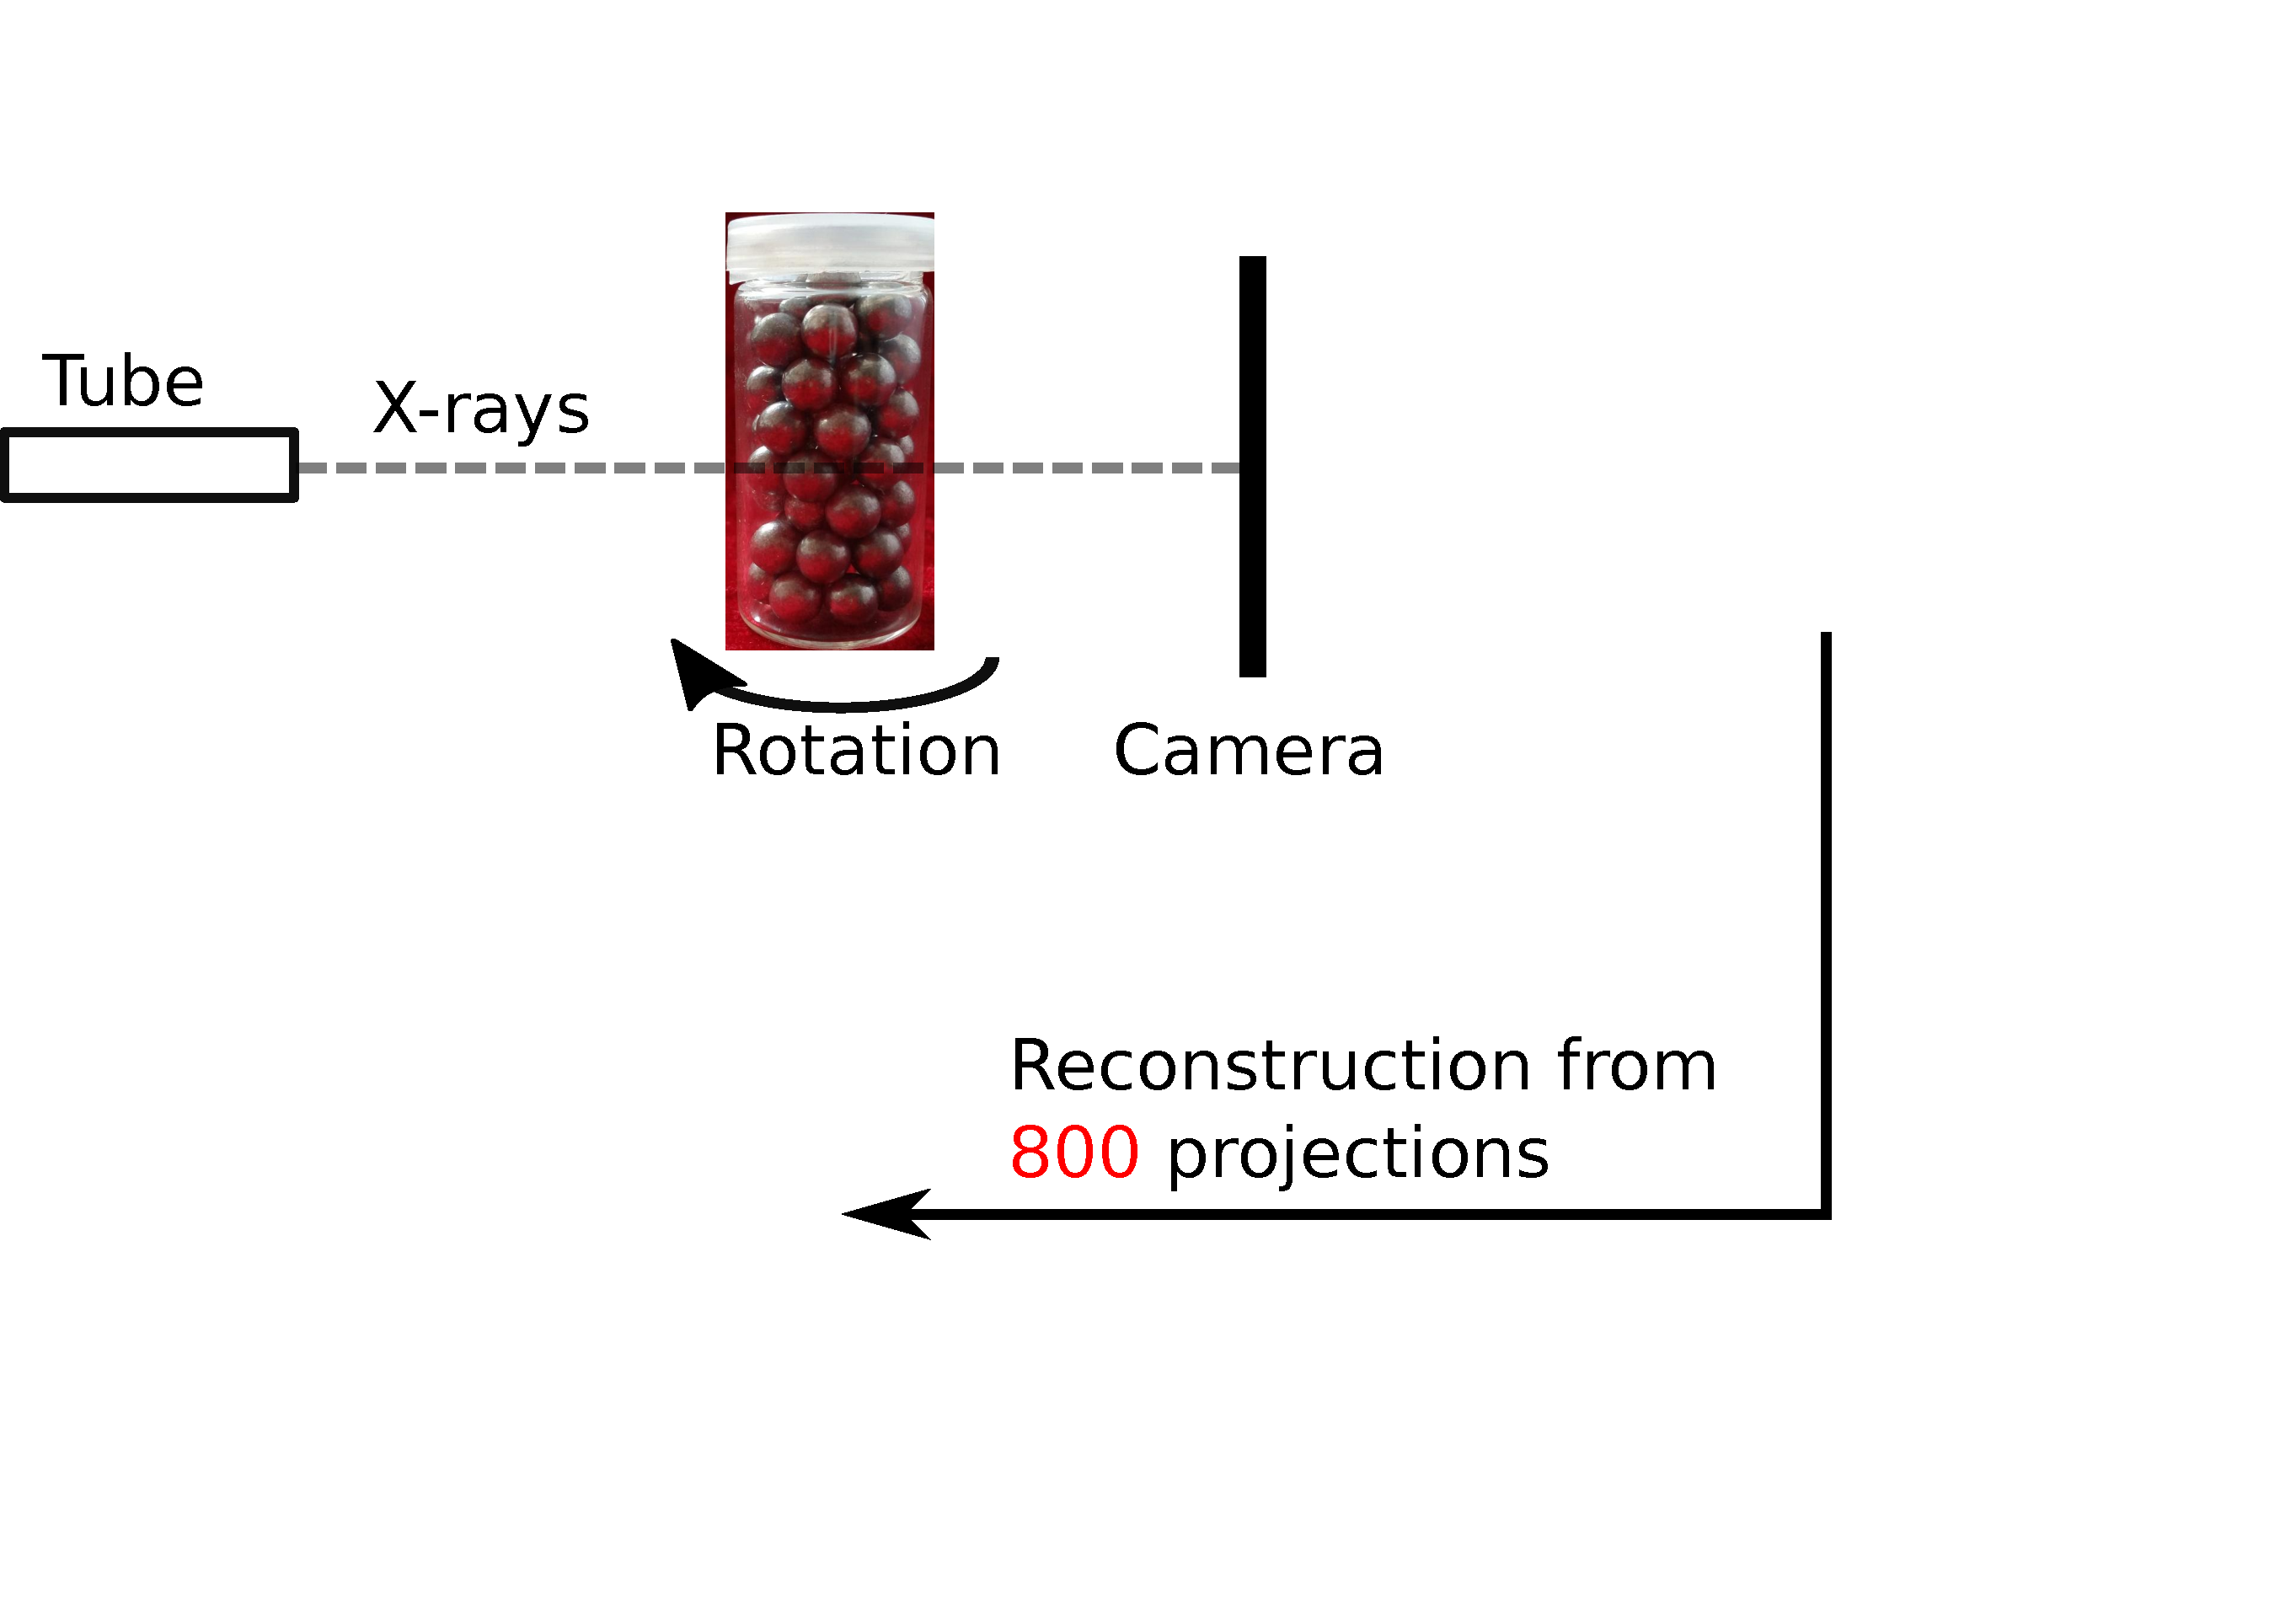
\includegraphics[width=\textwidth]{Sources/motivation/x-ray_setup_use.pdf}}
\end{textblock}

%% Video of Projections
\begin{textblock}{0.22}(0.45,0.05)
	\visible<1->{
	\centering
	Radiogram\\
	\fbox{
	\movie[width =\textwidth,loop]
	{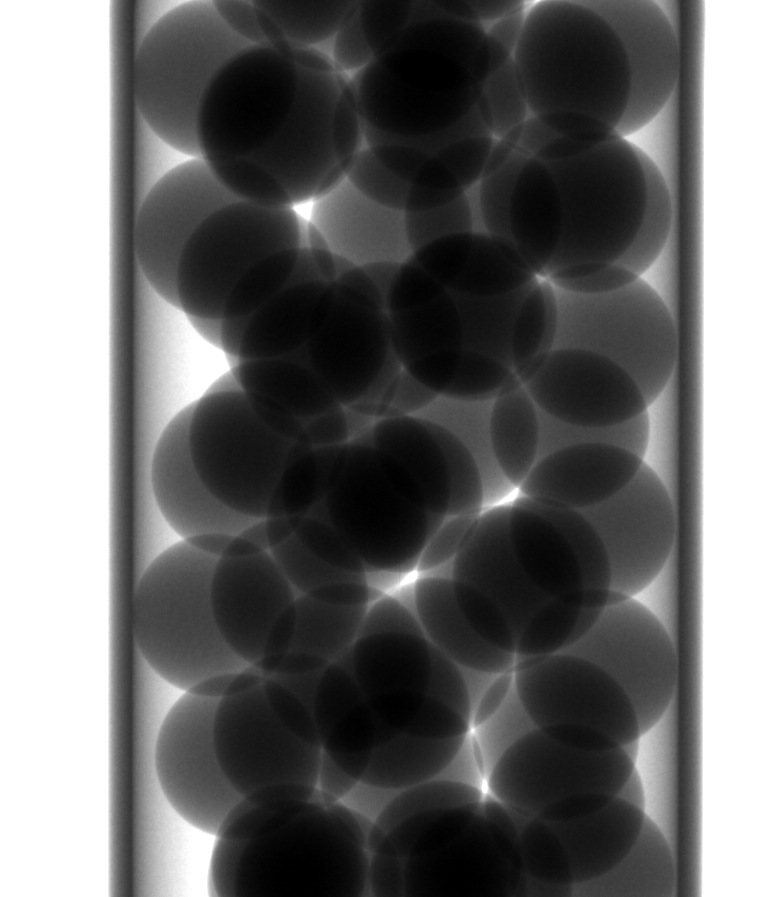
\includegraphics[width=\textwidth]{Sources/motivation/Projection0000.png}}
	{Sources/motivation/Projections360degree.avi}}}
\end{textblock}

\begin{textblock}{0.28}(0.7,0.25)
	\visible<1->{
	2D projections of 3D object\\
	\textcolor{blue1}{Short} acquisition time}
\end{textblock}

% Video of Tomography
\begin{textblock}{0.2}(0.05,0.48)
	\visible<2->{
	\centering
	Tomogram\\
	\movie[width =\textwidth,loop]
	{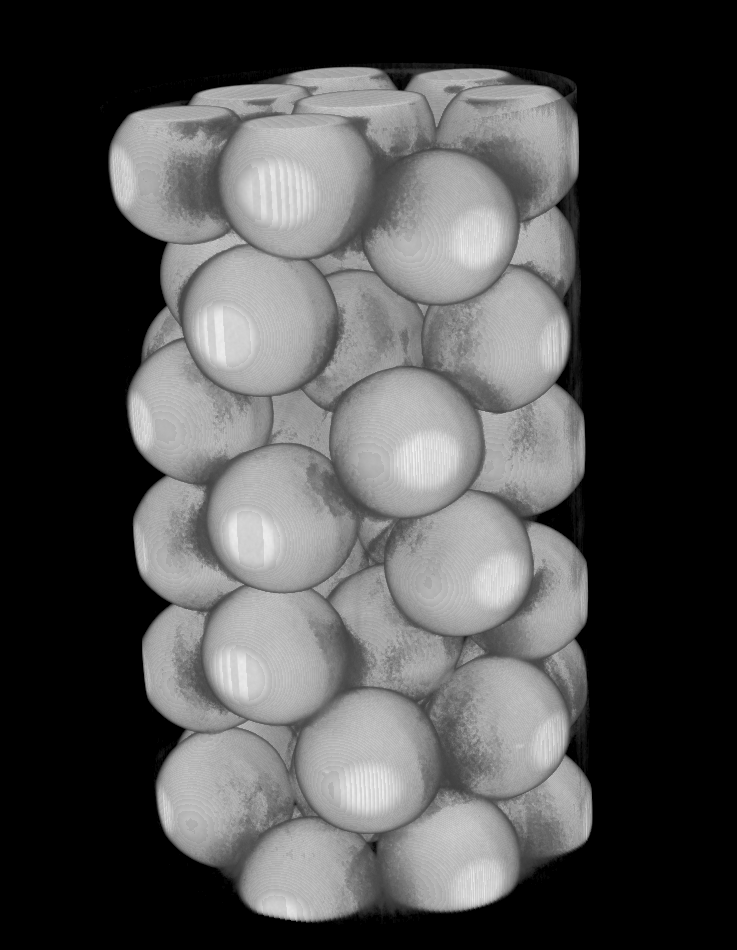
\includegraphics[width=\textwidth]{Sources/motivation/Images_tomo_movie0000.png}}
	{Sources/motivation/tomogram_360degree.avi}}
\end{textblock}

\begin{textblock}{0.5}(0.27,0.8)
	\visible<2->{
	Full 3D information\\
	\textcolor{red}{Long} acquisition time\\
	$\rightarrow$ static objects}
\end{textblock}

% Video of Tomography
\begin{textblock}{0.23}(0.72,0.5)
	\visible<3->{
		\centering
		\textcolor{blue1}{Dynamic} system\\
		\movie[width =\textwidth,loop]
		{
\includegraphics[width=\textwidth]{Sources/motivation/10000mul_per_min_0000.png}}
		{Sources/motivation/10000mul_per_min_original.avi}}
\end{textblock}
}


